\documentclass[11pt,a4paper]{article}

% Packages
\usepackage[utf8]{inputenc}
\usepackage[spanish, es-tabla]{babel}
\usepackage{caption}
\usepackage{listings}
\usepackage{minted}
\usepackage{adjustbox}
\usepackage[colorlinks=true]{hyperref}
\usepackage[shortlabels]{enumitem}
\usepackage{boldline}
\usepackage{amssymb, amsmath}
\usepackage{amsthm}
\usepackage[noend]{algpseudocode}
\usepackage[margin=1in]{geometry}
\usepackage{xcolor}
\usepackage{soul}
\usepackage{upgreek}

%\usemintedstyle{bw}

\decimalpoint

\hypersetup{
  colorlinks=magenta
}

% Meta
\title{Procesos Estocásticos\\ \Large{Ejercicios 2} }
\author{Antonio Coín Castro}
\date{\today}

% Custom
\providecommand{\abs}[1]{\lvert#1\rvert}
\setlength\parindent{0pt}
% Redefinir letra griega épsilon.
\let\epsilon\upvarepsilon
% Fracciones grandes
\newcommand\ddfrac[2]{\frac{\displaystyle #1}{\displaystyle #2}}
% Primera derivada parcial: \pder[f]{x}
\newcommand{\pder}[2][]{\frac{\partial#1}{\partial#2}}

\newcommand{\fx}{\frac{1}{\sqrt{2\pi}\sigma} e^{\frac{-(x-\mu)^2}{2\sigma^2}}}
\newcommand{\R}{\mathbb{R}}

\begin{document}
\maketitle

Consideramos la siguiente cadena de Markov:

\begin{figure}[h!]
  \centering
  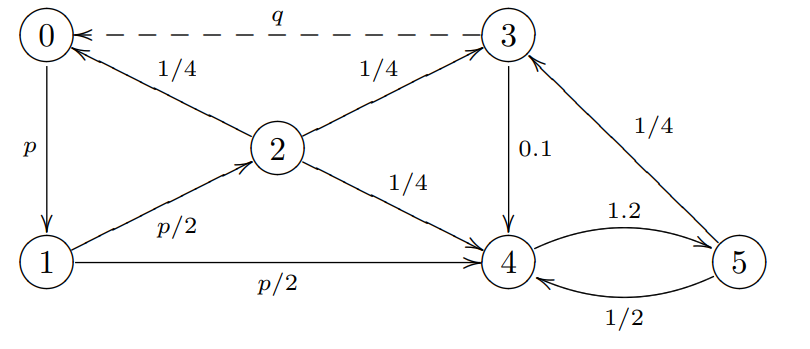
\includegraphics[width=.6\textwidth]{markov.png}
\end{figure}

Consideraremos siempre que $p=0.3$. La matriz de transición asociada es:

\[
P=\begin{pmatrix}
0.7 & 0.3 & 0 & 0 & 0 & 0\\
0 & 0.7 & 0.15 & 0 & 0.15 & 0\\
0.25 & 0 & 0.25 & 0.25 & 0.25 & 0\\
q & 0 & 0 & 0.9-q & 0.1 & 0\\
0 & 0 & 0 & 0 & 0.5 & 0.5\\
0 & 0 & 0 & 0.25 & 0.5 & 0.25
\end{pmatrix}
\]

\textbf{Ejercicio 1.} \textit{Simular el funcionamiento de la cadena y hacer una estimación de conjunto de $h_0^2$ y $h_0^5$ para $q=0.1$ y $q=0$}.\\

Escribimos un código para realizar esta simulación. En primer lugar, tenemos una clase que representa una cadena de Markov, construida a partir de la matriz de transición y de la distribución inicial. Dispone de métodos para computar la distribución teórica de los estados en cualquier instante $t$, para simular un paso de la cadena y para simular $t$ pasos. La clave a la hora de simular un paso es utilizar un valor aleatorio uniforme en $u \in [0,1]$, y avanzar al primer estado $k$ para el que se verifique que $u \leq \sum_{n=0}^k P_{mn}$, donde $m$ es el estado actual.

\begin{minted}{python}
import numpy as np
from scipy.stats import uniform
from scipy.optimize import nnls
import matplotlib.pyplot as plt

class MarkovChain:
    """
    This class represents a Markov chain via an initial state and a transition
    matrix. It keeps track of the probability of being in a certain state at
    any given time.
    """

    def __init__(self, P, m_ini):
        """ The state of the chain is represented by:
              - The total number of states, 'n'.
              - A transition matrix, 'P', of dimensions n x n.
              - The current state, 'm', indexed in [0, n-1].
              - The initial state, 'm_ini'.
              - The number of time instants that have passed, 'n_steps'.
              - An array that stores how many times each state has been visited,
                'state_count'. """

        self.P = P
        self.n = len(P[0])
        self.m_ini = m_ini
        self.m = m_ini
        self.n_steps = 1
        self.states_count = self.n * [0]
        self.states_count[self.m_ini] = 1  # We start at m_ini

    def theoretical_distribution(self, t):
        """ Return the theoretical distribution of the chain after t instants,
            starting from m_ini. """

        init_dist = [0] * self.n
        init_dist[self.m_ini] = 1
        return init_dist @ np.linalg.matrix_power(self.P, t)

    def step(self):
        """ Simulate a single step in the chain and return the new state. """

        u = uniform.rvs()
        self.m = np.where(np.cumsum(self.P[self.m]) >= u)[0][0]
        self.n_steps += 1
        self.states_count[self.m] += 1
        return self.m

    def steps(self, t):
        """ Perform T steps in the chain and return the new state. """

        for _ in range(t):
            self.step()
        return self.m
\end{minted}

Entonces, podemos definir una función para calcular el valor de $h_{m_0}^m$ de forma empírica, simplemente simulando $n$ cadenas independientes hasta un número fijo $t$ de pasos, y viendo en cuántas de ellas se llega al estado $k$ partiendo de $m$.

\begin{minted}{python}
def empirical_h(P, m_ini, m, t, n):
    """ Compute the empirical hitting probability of m with n independent
        executions of t iterations of the chain (P, m_ini). """

    if m_ini == m:
        return 1.0
    hits = 0
    for i in range(n):
        MC = MarkovChain(P, m_ini)
        MC.steps(t)
        if MC.states_count[m] > 0:
            hits += 1
    return hits / n
\end{minted}

Podemos entonces definir en el código nuestras matrices de transición, $P_1$ con $q=0$ y $P2$ con $q=0.1$, y realizar las simulaciones pertinentes.

\begin{minted}{python}
# Number of independent simulations and steps in each one
n = 1000
t = 1000

print("\nEMPIRICAL PROBABILITIES")
print(f"Simulating {n} independent chains up to {t} steps...\n")
print("--- Hitting probability ---")
emp_h02_1 = empirical_h(P1, 0, 2, t, n)
emp_h05_1 = empirical_h(P1, 0, 5, t, n)
print("With q = 0.0:")
print("  h02 =", emp_h02_1)
print("  h05 =", emp_h05_1)
emp_h02_2 = empirical_h(P2, 0, 2, t, n)
emp_h05_2 = empirical_h(P2, 0, 5, t, n)
print("With q = 0.1:")
print("  h02 =", emp_h02_2)
print("  h05 =", emp_h05_2)
\end{minted}

Simulando 1000 cadenas independientes hasta 1000 iteraciones (con semilla $42$), obtenemos los siguientes resultados:

\begin{verbatim}
--- Hitting probability ---
With q = 0.0:
  h02 = 0.494
  h05 = 1.0
With q = 0.1:
  h02 = 1.0
  h05 = 1.0
\end{verbatim}

\textbf{Ejercicio 2}. \textit{Simular el funcionamiento de la cadena y hacer una estimación de conjunto de $k_0^2$ y $k_4^2$ para $q=0.1$ y $q=0$}.\\

Definimos esta vez una función para calcular $k_{m_0}^m$ de forma empírica, simulando $n$ cadenas independientes hasta un número $t$ de iteraciones, y contando cuál ha sido la primera vez que se alcanza el estado $m$. Si en alguna de las simulaciones no se consigue alcanzar el estado, supondremos que $k_{m_0}^m=\infty$. En otro caso, devolvemos la media de los \textit{hitting times}.

\begin{minted}{python}
def empirical_k(P, m_ini, m, t, n):
    """ Compute the empirical expected hitting time of m with n independent
        executions of t iterations of the chain (P, m_ini). """

    if m_ini == m:
        return 0.0
    hit_time = [0.0] * n
    for i in range(n):
        MC = MarkovChain(P, m_ini)
        for tt in range(t):
            if MC.step() == m:
                hit_time[i] = tt + 1
                break
    return np.Infinity if 0.0 in hit_time else np.mean(hit_time)
\end{minted}

Una vez hecho esto, ejecutamos las simulaciones, obteniendo los siguientes resultados:

\begin{verbatim}
With q = 0.0:
  k02 = inf
  k42 = inf
With q = 0.1:
  k02 = 42.201
  k42 = 76.304
\end{verbatim}

Observamos que los casos en los que obtenemos $k=\infty$ tiene sentido que sea así, ya que el correspondiente valor de $h$ es menor que $1$. En efecto, si recordamos:

\[
k_{m_0}^m = \mathbb E[H_{m_0}^m]= \sum_{t < \infty} t P_{m_0}(H_{m_0}^m=t) + \infty P_{m_0}(H_{m_0}^m = \infty),
\]

donde por convención $\infty\cdot 0=0$. Así, si $P_{m_0}(H_{m_0}^m = \infty) > 0$ (es decir, $h_{m_0}^m = P_{m_0}(H_{m_0}^m<\infty)<1$), tendremos que $k_{m_0}^m = \infty$.\\

\textbf{Ejercicio 3}. \textit{Usar el sistema de ecuaciones lineales oportuno para determinar los valores teóricos correspondientes a las cantidades estimadas y comparar con los valores determinados por medio de la simulación.}\\

Sabemos que el vector de \textit{hitting probabilities} viene dado como la solución minimal no negativa del sistema de ecuaciones:

\[
\begin{cases}
  h_m^{\mathcal A} = 1, & m \in \mathcal A\\
  h_m^{\mathcal A} = \sum_{n} P_{mn}h_n^{\mathcal A}, & m \notin \mathcal A.
\end{cases}
\]

Observamos que se trata de un sistema lineal de la forma $Ax=b$. Podemos escribir la matriz $A$ en términos de $P$, y el vector $b$ será un vector de ceros con un $1$ en la posición que nos interese. Para resolverlo, utilizamos la función \verb|nnls| de \verb|scipy|, que nos permite encontrar la solución minimal y no negativa de un sistema lineal. Así, para los casos en los que nos queden ecuaciones con infinitas soluciones del tipo $h_m=h_m$, se elegirá $h_m=0$ al ser el valor no negativo más pequeño.

\begin{minted}{python}
def theoretical_h(P, m):
    """ Compute the theoretical hitting probability of m on the chain (P). """

    n = len(P[0])
    A = -P
    A += np.diag(np.ones(n))
    b = np.zeros(n)
    b[m] = 1
    A[m] = b
    return nnls(A, b)[0]
\end{minted}

Si ejecutamos esta función para los diferentes valores de $q$, obtenemos una tabla como la que aparece a continuación. Observamos que son valores muy cercanos a los que obtuvimos con nuestra simulación. De hecho, coincide exactamente para todos excepto para $h_0^2$ con $q=0.0$, donde habrían hecho falta algunas simulaciones extra para acercarse aún más a la probabilidad de $0.5$. Mostramos también el valor de $h_4^2$, que nos servirá para cálculos posteriores.

\begin{table}[h!]
  \centering
  \begin{tabular}{c|c|c|c}
    \textbf{q} & \textbf{$h_0^2$} & \textbf{$h_0^5$} & \textbf{$h_4^2$}\\ \hline
    0.0 & 0.5 & 1.0 & 0.0 \\
    0.1 & 1.0 & 1.0 & 1.0\\
  \end{tabular}
\end{table}

Para el caso de los valores de $k$, sabemos también que son la solución minimal no negativa del sistema de ecuaciones:

\[
\begin{cases}
  k_m^{\mathcal A} = 0, & m \in \mathcal A\\
  k_m^{\mathcal A} = 1 + \sum_{n \notin A} P_{mn}k_n^{\mathcal A}, & m \notin \mathcal A.
\end{cases}
\]

En este caso podemos hacer algunas simplificaciones. Por ejemplo, sabemos que si $h<1$, entonces la correspondiente $k$ es $\infty$ (lo vimos en el ejercicio anterior). En nuestro caso, para $q=0$ se tiene $h_0^2<1$ y también $h_4^2<1$, luego necesariamente $k_0^2=\infty$ y $k_4^2=\infty$.\\

Para el caso $q=0.1$, podemos resolver el sistema asociado del mismo modo que hicimos antes, siempre y cuando ninguna de las $k$ que intervengan sea $\infty$.

\begin{minted}{python}
def theoretical_k(P, m):
    """ Compute the theoretical expected hitting time of m on the chain (P),
       given that they are all finite. """

    n = len(P[0])
    A = -P
    A += np.diag(np.ones(n))
    b = np.ones(n)
    b[m] = 0
    A[m] = np.logical_not(b)
    return nnls(A, b)[0]
\end{minted}{python}

Ejecutando esta función, y teniendo en cuenta los cálculos anteriores, obtenemos la siguiente tabla de resultados:

\begin{table}[h!]
  \centering
  \begin{tabular}{c|c|c}
    \textbf{q} & \textbf{$k_0^2$} & \textbf{$k_4^2$}\\ \hline
    0.0 & \infty & \infty\\
    0.1 &  43.33 & 73.33
  \end{tabular}
\end{table}

Vemos que de nuevo los valores simulados en el ejercicio anterior coinciden más o menos con los valores teóricos, por lo que podemos afirmar que nuestra simulación es buena. Notamos que el caso en que $k=\infty$ en principio no se puede simular. En nuestra simulación hemos establecido un límite de iteraciones para el que consideramos que si no se ha alcanzado un nodo en esa simulación, ya no se alcanzará. Lo ideal sería, si la capacidad de cómputo lo permite, aumentar ese límite todo lo posible para aumentar nuestra creencia. Sin embargo, nunca podremos estar seguros al $100\%$ si no calculamos el valor teórico.\\

\textbf{Ejercicio 4}. \textit{Para el caso $q=0.1$, dibujar la gráfica de la función $g(t)=\mathbb P[H_0^4 = t]$.}\\

Nos preguntan por la función que modela la probabilidad de que cada instante sea el \textit{first hitting time} para el estado $4$, partiendo del estado $0$. Para descomponer esta probabilidad en el tiempo, podemos utilizar la siguiente idea: si $t>1$, para que el \textit{first hitting time} de un estado $i$ a un estado $j$ sea $t$, la cadena debe moverse de $i$ a $k\neq j$ en un paso, y entonces el \textit{first hitting time} de $k$ a $j$ debe ser $t-1$. A partir de esto, denotando $f^{(t)}_{ij}=\mathbb P[H_i^j = t]$, obtenemos la siguiente recurrencia:

\[
\begin{cases}
f_{ij} = P_{ij}\\
f^{(t)}_{ij} =  \sum_{k\neq j} P_{ik}f_{kj}^{(t-1)}, \quad t > 1.
\end{cases}
\]

Implementamos esta relación en una función:

\begin{minted}{python}
def plot_first_hitting_time(P, m_ini, m, tmax=100):
    """ Plot the (theoretical) graph of P[H_{m_ini}^{m} = t]. """

    n = len(P[0])
    idx = list(np.arange(m)) + list(np.arange(m + 1, n))
    g = np.zeros(tmax + 1)
    f = P[idx, m]
    g[0] = 0
    g[1] = f[m_ini]  # first step
    for t in range(2, tmax + 1):
        f = [f @ P[i, idx] for i in idx]
        g[t] = f[m_ini]
    return g
\end{minted}

Al ejecutarla, obtenemos la siguiente gráfica:
\begin{figure}[h!]
  \centering
  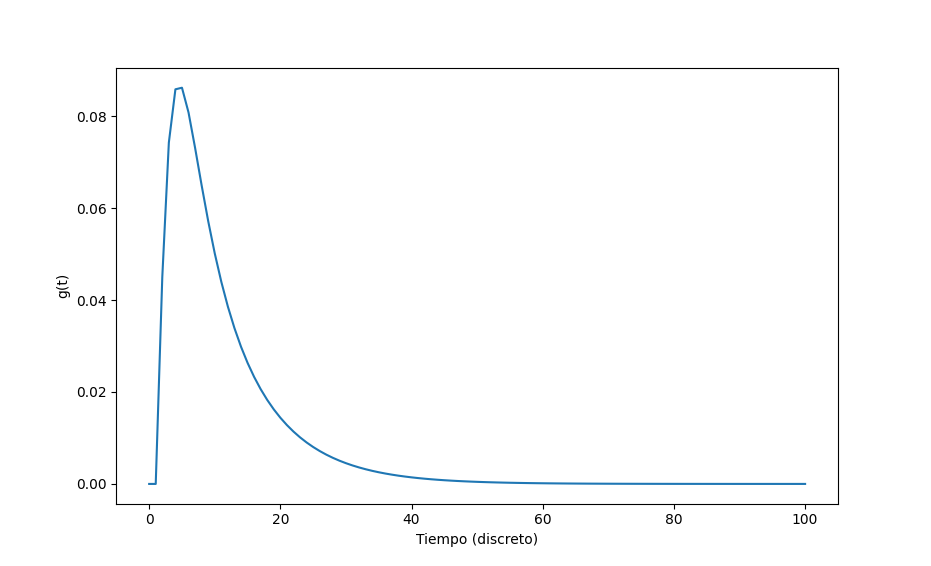
\includegraphics[width=.9\textwidth]{ej4.png}
  \caption{Gráfica de $g(t)=\mathbb P[H_0^4=t].$}
\end{figure}

Podemos interpretar esta gráfica fácilmente. En $t=0$ estamos en el estado $0$, luego la probabilidad que nos interesa es $0$. La probabilidad de que tras el primer movimiento alcancemos el estado $4$ es también 0, ya que es imposible llegar de $0$ a $4$ en un solo movimiento. Después, la probabilidad de alcanzar el $4$ por primera vez va aumentando; al principio es difícil, pero conforme aumentamos el tiempo va aumentando la probabilidad. Llega un momento en que $g(t)$ llega a su máximo, forma una especie de meseta, y luego comienza a descender, ya que conforme avanza la cadena es cada vez menos probable que pasemos por $4$ por primera vez.\\

\textbf{Ejercicio 5}. \textit{Afirmo que $H_0^4 < H_0^5$ siempre. ¿Es cierto?}\\

Sí es cierto, ya que si observamos la cadena, para llegar al estado $5$ es imprescindible pasar por el estado $4$, luego como mínimo llegaremos al estado $5$ un instante de tiempo después de haber llegado al $4$.
\end{document}
